\documentclass{article}

\usepackage{listings}
\usepackage{parskip}
\setlength{\parskip}{0pt}
\usepackage{graphicx}
\graphicspath{{./images/}}
\usepackage{float}

\title{Pd-Ofelia suficiente para te salvar}
\author{Haruo}
\date{}

\begin{document}

\maketitle

\section{Introdução}

% \section{Objeto \texttt{ofelia function}}

% \section{Objeto \texttt{ofelia define}}

\section{Scripts \texttt{.lua}}

A biblioteca Ofelia registra automaticamente funções nomeadas como \texttt{ofelia.*} para serem usadas como \textbf{manipuladores de mensagens} no Pure Data.\lstset{inputencoding=utf8/latin1}
Por exemplo:

Crie um arquivo \texttt{meuScript.lua} e defina a seguinte função:

\begin{center}
  \begin{lstlisting}
  function ofelia.minhaMensagem();
  print('Executei a funcao minhaMensagem!');
  end;
  \end{lstlisting}
\end{center}

Crie um patch em Pure Data nomeado \texttt{meuPatch.pd} no mesmo diretório do script e adicione os seguintes objetos:

\begin{figure}[h]
  \centering
  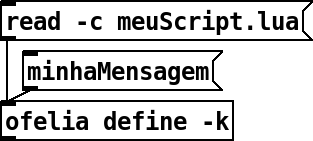
\includegraphics[width=100pt]{passo1.png}
\end{figure}

Clique na mensagem \texttt{read -c meuScript.lua} para carregar o script no Pure Data. Clique na mensagem \texttt{minhaMensagem} para \textbf{executar a função do script com o nome da mensagem mandada}. A função \texttt{ofelia.minhaMensagem()} será executada e a mensagem \texttt{Executei a funcao minhaMensagem!} será impressa no console.

\subsection{A variável global \texttt{M}}

Continuando com o nosso exemplo, complemente seu patch adicionando um objeto \texttt{bang} da seguinte maneira:

\begin{figure}[H]
  \centering
  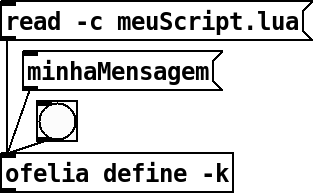
\includegraphics[width=100pt]{passo2.png}
\end{figure}

Como fazer esse objeto \texttt{bang}, ao ativado, chamar alguma função do script \texttt{meuScript.lua}?

Podemos fazer isso adicionando a seguinte função ao script:

\begin{center}
  \begin{lstlisting}
  function M.bang();
  print('Executei a funcao ao ativar o bang!');
  end;
  \end{lstlisting}
\end{center}

% "M" is the name of a module table that exists in each "ofelia define" object which includes built-in functions such as "M.bang()" function. You can add any variables or functions to the module.
Perceba que não definimos \texttt{M} em lugar algum em nosso script.
Na verdade, \texttt{M} é um módulo-tabela que existe em todo objeto \texttt{ofelia define} e inclui funções embutidas como a função \texttt{M.bang()} (detalhes das funções embutidas podem ser encontradas na sessão \ref{subsection:funcoes-embutidas} deste documento).
Além disso, é possível definir variáveis e funções personalizadas no módulo \texttt{M}.

\subsection{Funções embutidas}\label{subsection:funcoes-embutidas}

O Ofelia oferece algumas funções embutidas.

\subsubsection{\texttt{M.*()}}

Algumas das funções embutidas com o módulo \texttt{M} são:

\begin{center}
  \begin{lstlisting}
  function M.new();
  end;
  ;
  function M.free();
  end;
  ;
  function M.bang();
  print("got bang");
  end;
  ;
  function M.float(f);
  print("got float : " .. f);
  return f;
  end;
  ;
  function M.symbol(s);
  print("got symbol : " .. s);
  end;
  ;
  function M.list(l);
  for i=1, #l do;
  print("got list : " .. l\[i\]);
  end;
  end;
  ;
  function M.pointer(p);
  print("got pointer : " .. p.r, p.g, p.b);
  end;
  \end{lstlisting}
\end{center}

\subsubsection{\texttt{ofelia.perform()}}

Defina uma função \texttt{ofelia.perform()} para ser executada a cada ciclo DSP.

\end{document}